\chapter{Implementacja}
\label{cha:implementation}

\section{Architektura rozwiązania}

\begin{figure}[!ht]
	\begin{center}
		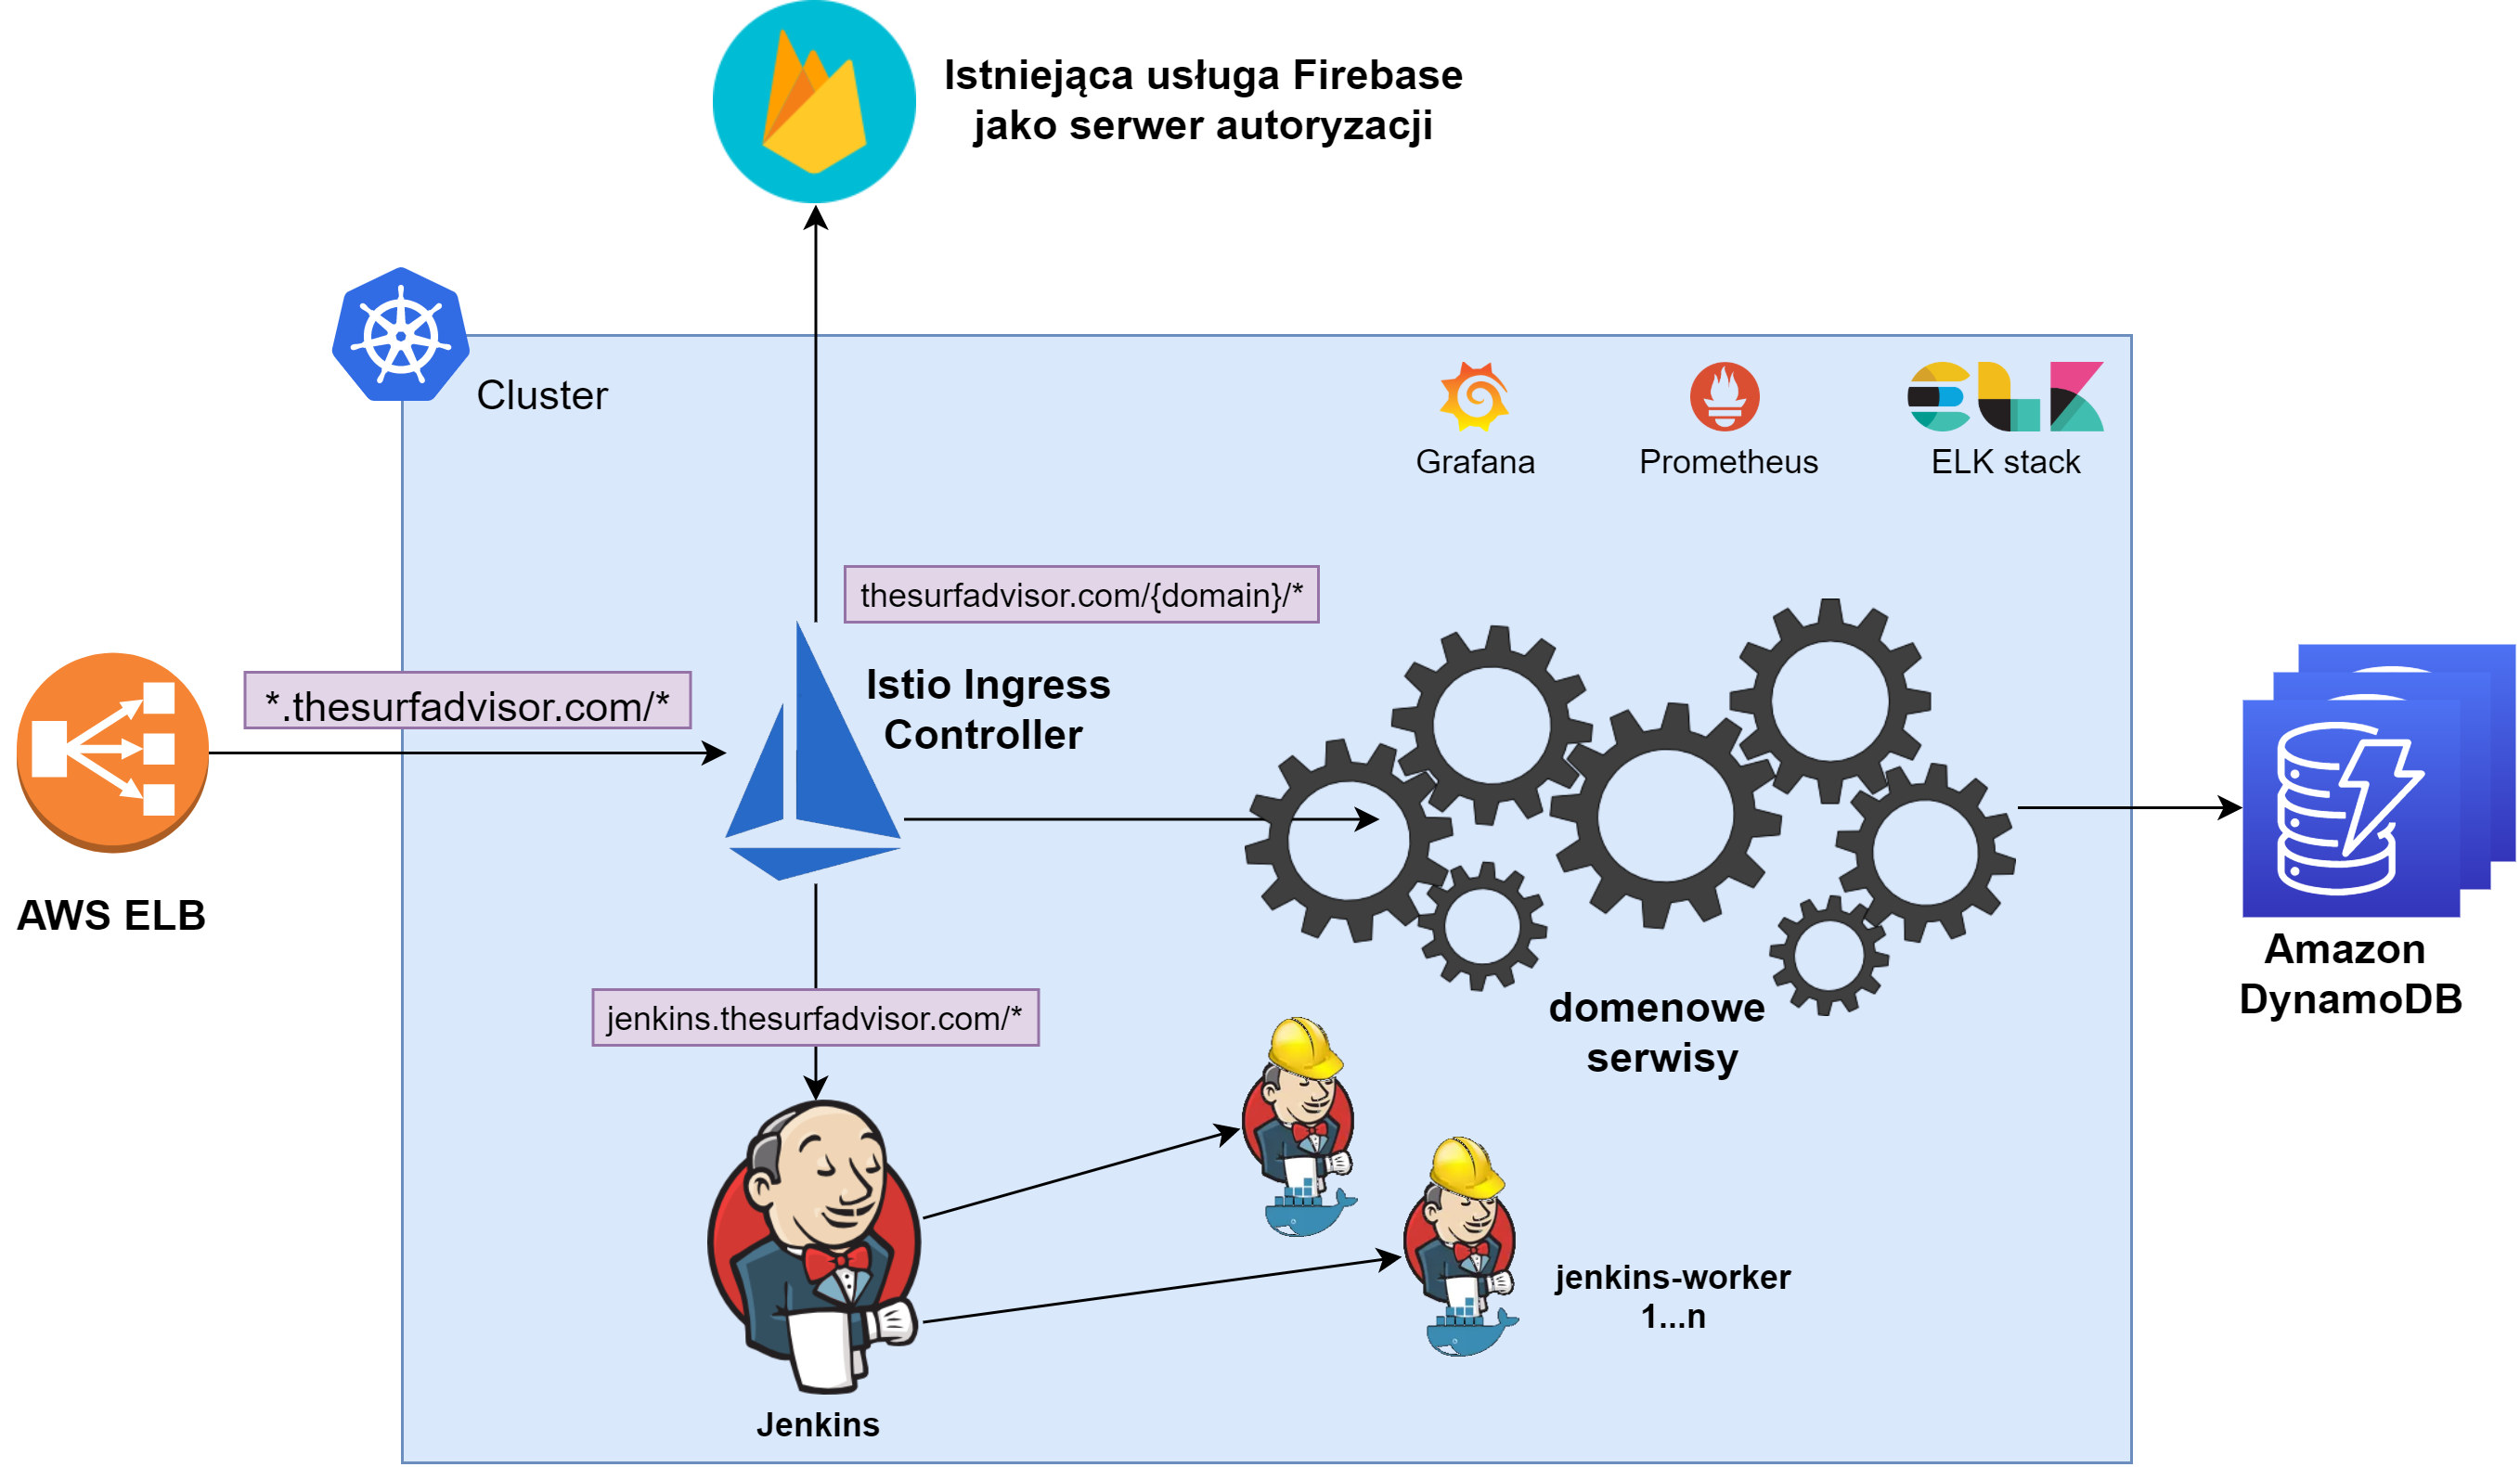
\includegraphics[width=1\textwidth]{img/surf-cluster}
	\end{center}
	\caption{Cluster nowych usług SurfAdvisor}
\end{figure}

\cw{Cluster} nowych usług SurfAdvisor w spoczynku składa się z: 

\begin{itemize}
    \item
    1 x master \cw{Node} - EC2 \textbf{m3.medium} \emph{(1 vCPU \& 3.75 GiB RAM)}

    \item
    2 x worker \cw{Node} - EC2 \textbf{t3.medium} \emph{(2 vCPU \& 4 GiB RAM)}
\end{itemize} 

W przypadku zwiększenia natężenia ruchu liczba \cw{Node}'ów jest skalowana by sprostać wymaganiom.
Pod globalnie dostępną domeną \textbf{thesurfadvisor.com} kryje się \emph{Load Balancer} utrzymywany przez AWS.
Stanowi on jedyny punkt dostępu, cały ruch jest następnie obsługiwany przez Istio \emph{Ingress Controller}.
Autoryzacja zintegrowana jest z istniejącym systemem Firebase. Każdy domenowy serwis uderza do własnej bazy danych DynamoDB.

Jako administrator możemy się dostać do subdomen takich jak:

\begin{itemize}
    \item
    \emph{\textbf{jenkins}.thesurfadvisor.com}\\ 
    Jenkins \emph{WEB UI} pracującego wewnątrz \cw{Cluster}'a

    \item
    \emph{\textbf{grafana}.thesurfadvisor.com}\\
    Grafana \emph{WEB UI} śledząca metryki stanu technicznego

    \item
    \emph{\textbf{kibana}.thesurfadvisor.com}\\
    Kibana \emph{WEB UI} do wygodnego przeszukiwania logów
\end{itemize} 



\section{Aplikacje biznesowe}

\begin{figure}[!ht]
	\begin{center}
		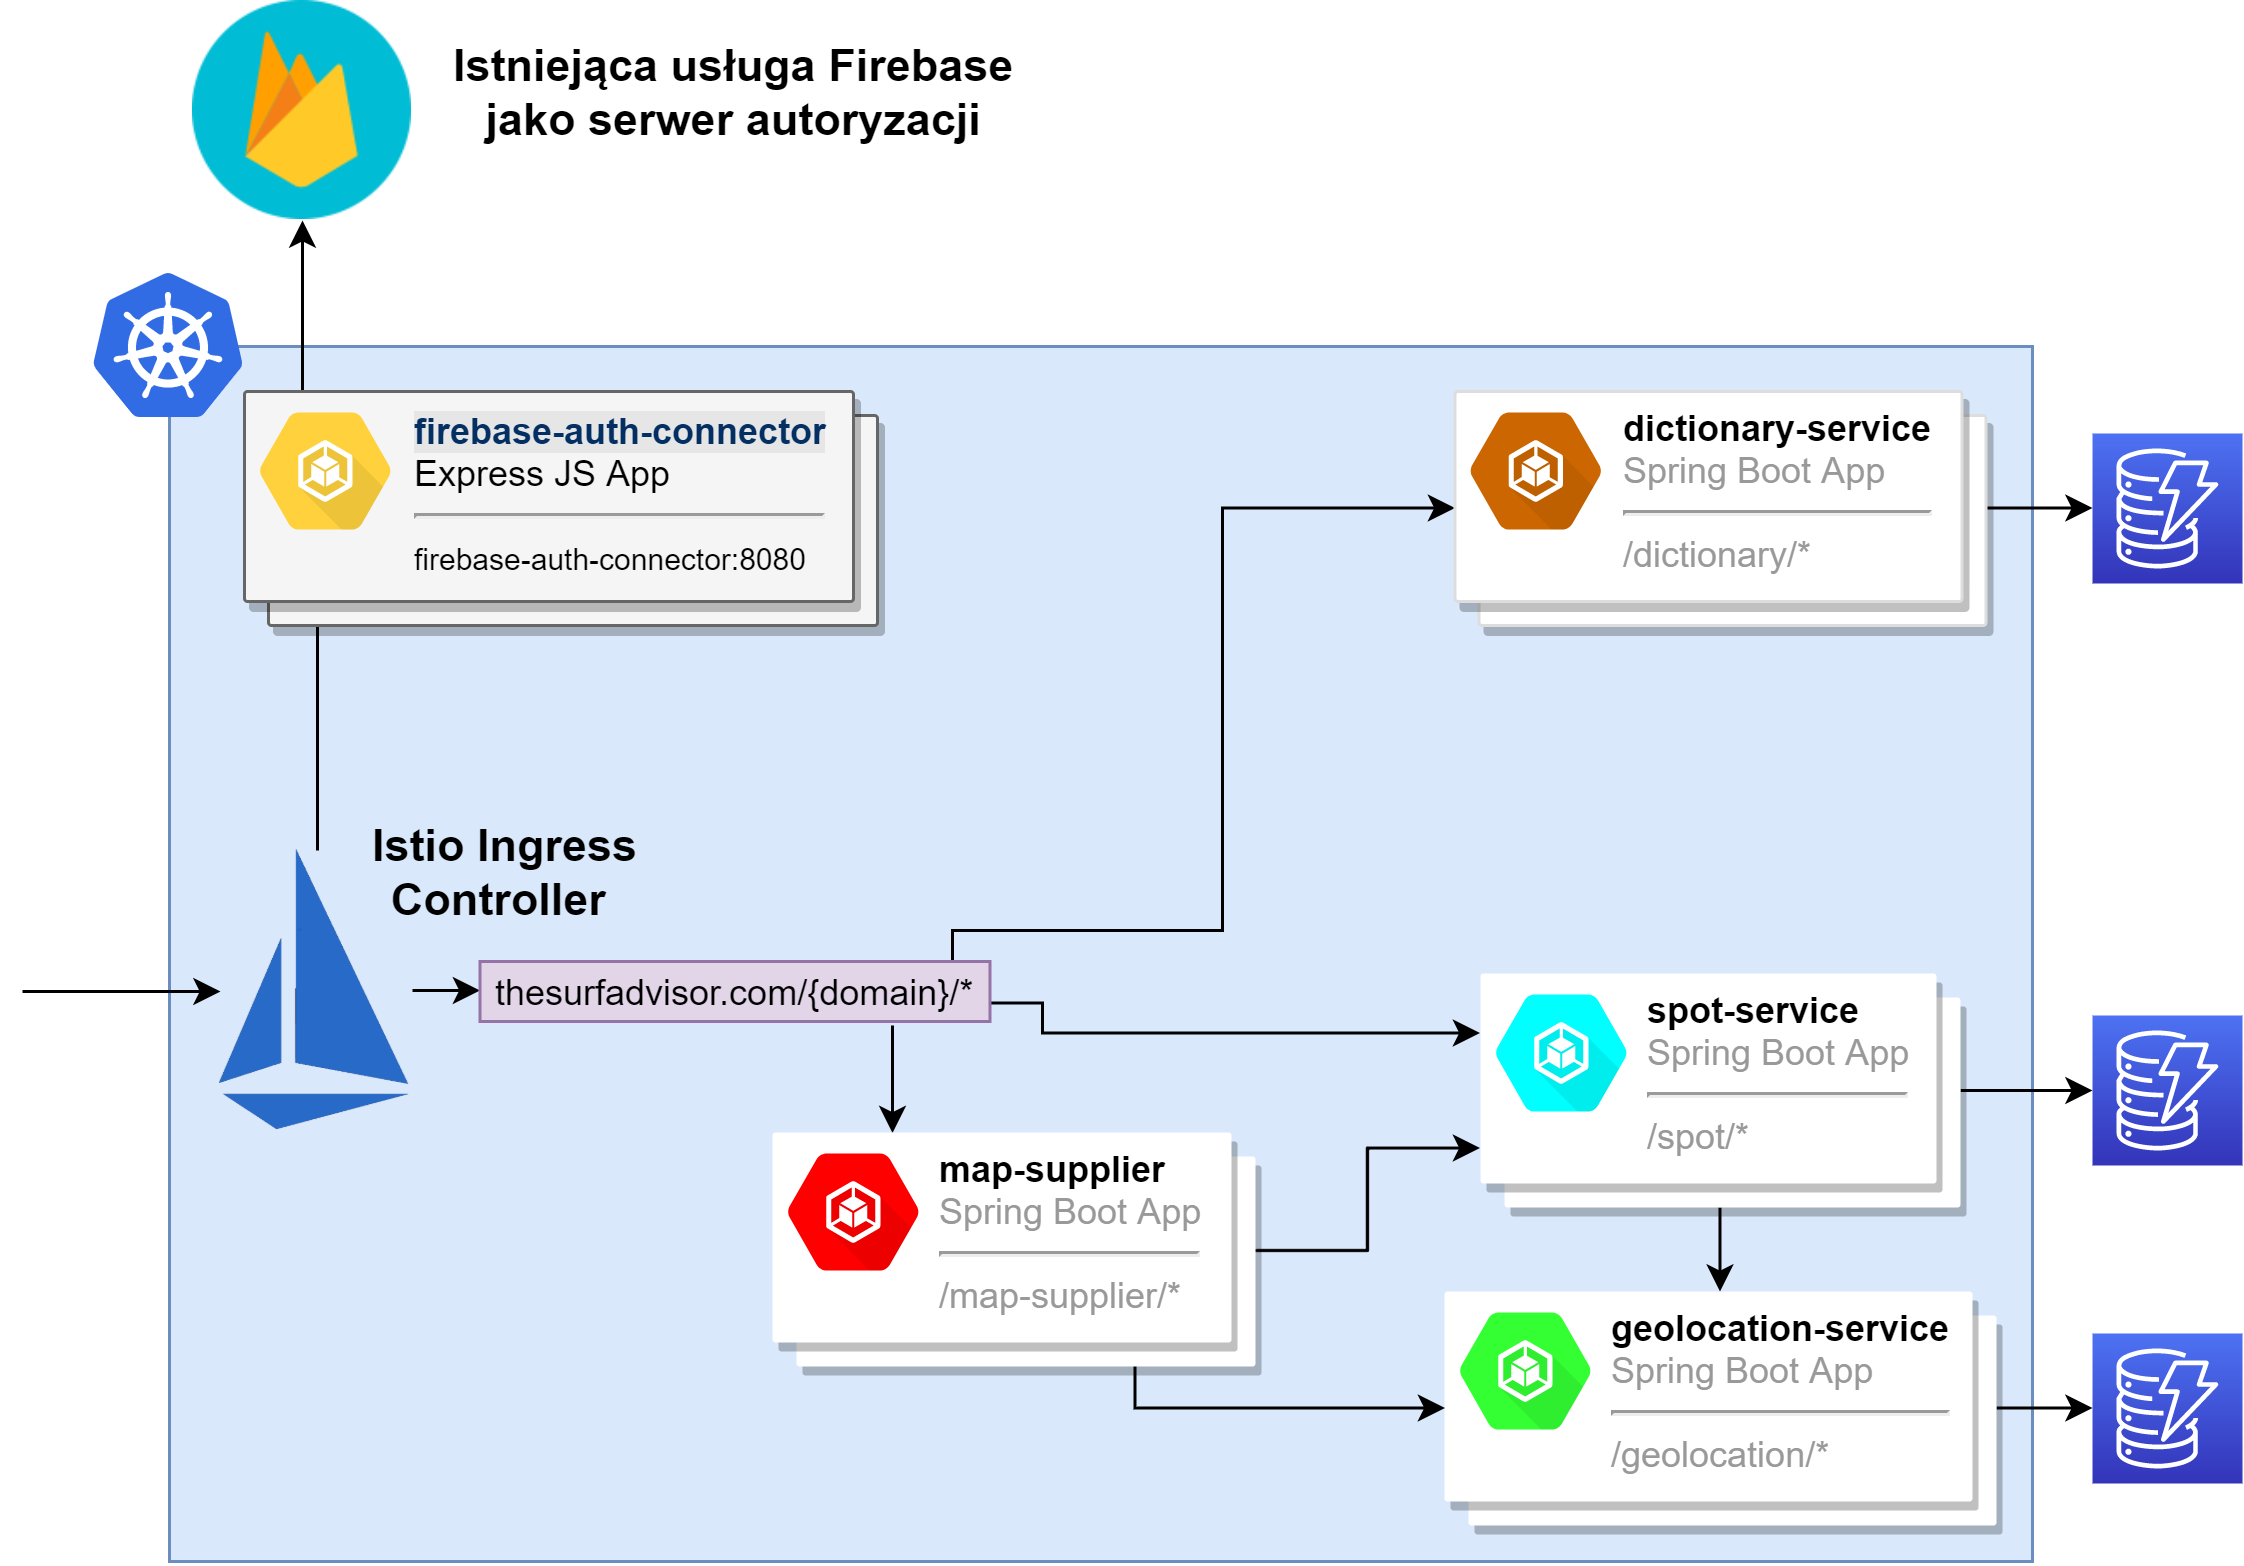
\includegraphics[width=1\textwidth]{img/surf-services}
	\end{center}
	\caption{Zbliżenie na domenowe serwisy SurfAdvisor}
\end{figure}

\begin{itemize}
    \item
    \textbf{firebase-auth-connector}\\ 
    Warstwa pośrednia pomiędzy Istio \emph{Ingress Controller} a istniejącym serwisem Firebase.
    
    \item
    \textbf{dictionary-service}\\ 
    Repozytorium literałów wyświetlanych w aplikacji mobilnej.

    \item
    \textbf{geolocation-service}\\ 
    Wiedza o położeniu obiektów na kuli ziemskiej.

    \item
    \textbf{spot-service}\\ 
    Atlas spotów - miejsc do uprawiania sportu wodnego.

    \item
    \textbf{map-supplier}\\ 
    Agreguje resztę serwisów związanych z mapą, by wydajniej obsłużyć aplikacje mobilną.
\end{itemize} 




\section{IaC - Infrastructure as Code}

Jest to podejście do zarządzania infrastrukturą \emph{(siecią, wirtualnymi maszynami, kontenerami etc.)} poprzez pliki tekstowe, 
których treść w sposób jednoznaczny definiuje potrzebne zasoby. 
Taką deklaratywną formę konfiguracji bardzo łatwo można śledzić poprzez ten system kontroli wersji co ten używany wokół kodu aplikacji.
IaC jest odpowiedzią na problem różnic pomiędzy środowiskami narastającymi jeszcze bardziej z czasem, jakie powodowały ich manualne imperatywne modyfikacje.
Założeniem IaC jest \textbf{idempotentność} wdrożeń definicji z plików - za każdym razem rezultatem ma być takie samo środowisko \cite{iac-ms}.

W projekcie realizuje tę koncepcję stawiając cały system w czterech krokach. 
Pierwsze trzy stawiają \cw{Cluster} na AWS, są w pełni zautomatyzowane: \emph{CloudFormation}, \emph{Kops} i \emph{Kubernetes}.
Ostatni wdraża domenowe aplikacje, wymaga paru kliknięć w konsoli webowej \emph{Jenkins}'a. 

\subsection{CloudFormation}
\label{iac:cf}

\begin{figure}[!ht]
	\begin{center}
		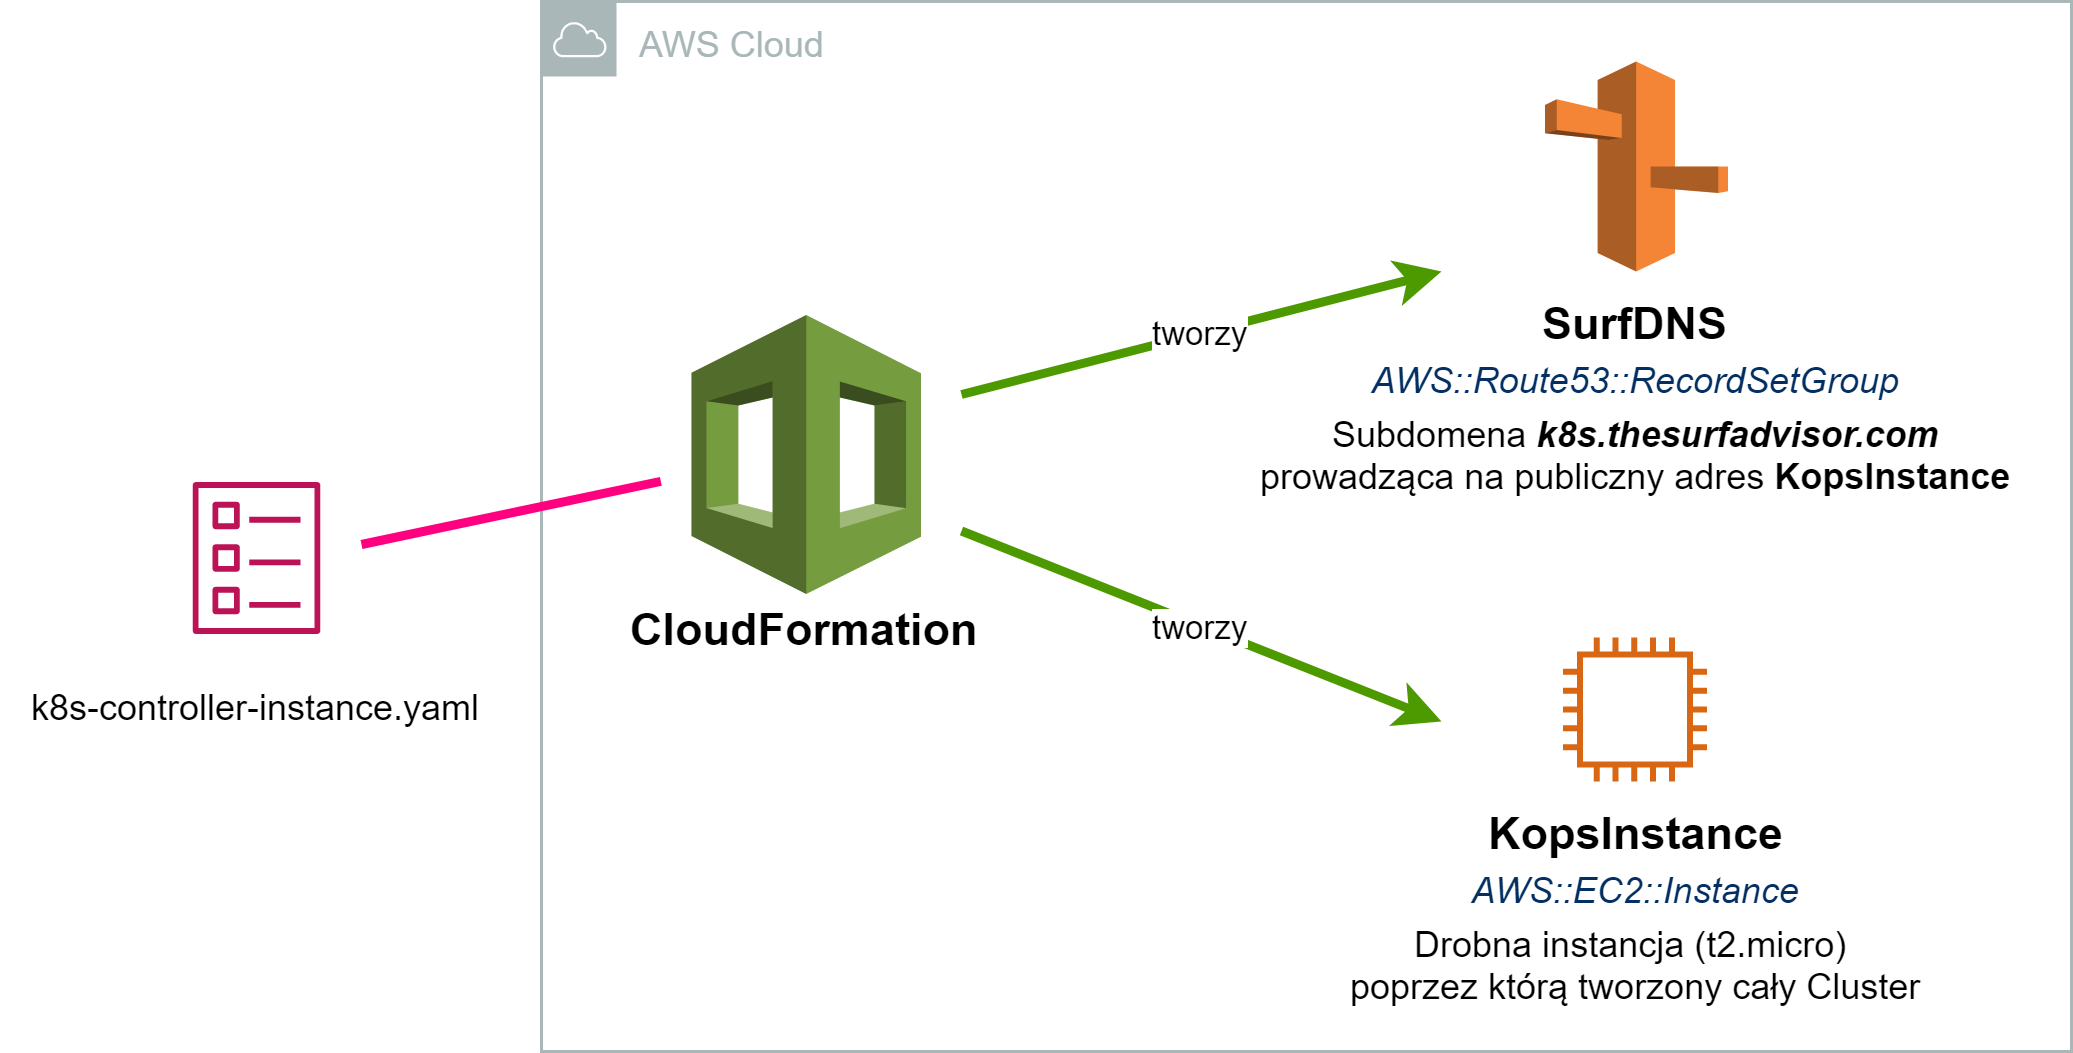
\includegraphics[width=0.9\textwidth]{img/IAC-step1}
	\end{center}
	\caption{Inicjacja Cluter'a SurfAdvisor - 1. CloudFormation}
\end{figure}

Najistotniejszym plikiem CloudFormation w projekcie jest ten inicjujący drobną instancję przeznaczoną do zarządzania docelowym \cw{Cluster}'em.
Plik \cw{k8s-controller-instance.yaml} definiuje głównie: 

\begin{itemize}
    \item
    \textbf{KopsInstance} - drobna instancja linuxa 
    
    \item
    \textbf{SurfDNS} - subdomena oszczędzająca znajomości dokładnego adresu IP \emph{(np. w razie potrzeby ssh)}
\end{itemize} 

Kluczowe znaczenie ma możliwość definicji \emph{\textbf{UserData}} - skryptu \emph{bash} wykonywanego zaraz po starcie instancji. 
Zdefiniowałem w nim polecenia:

\begin{itemize}
    \item
    ściągnięcia dalszych instrukcji \emph{bash} z S3

    \item
    instalacji potrzebnych narzędzi \emph{(kops, kubectl, helm)}
    
    \item
    zbudowania \cw{Cluster}'a poprzez \emph{kops} \emph{(\ref{iac:kops})}

    \item
    wdrożeniu pomocniczych \cw{Service}'ów poprzez \emph{kubectl} \& \emph{helm} \emph{(\ref{iac:kubectl})}
\end{itemize} 

\subsection{Kops}
\label{iac:kops}

\begin{figure}[!ht]
	\begin{center}
		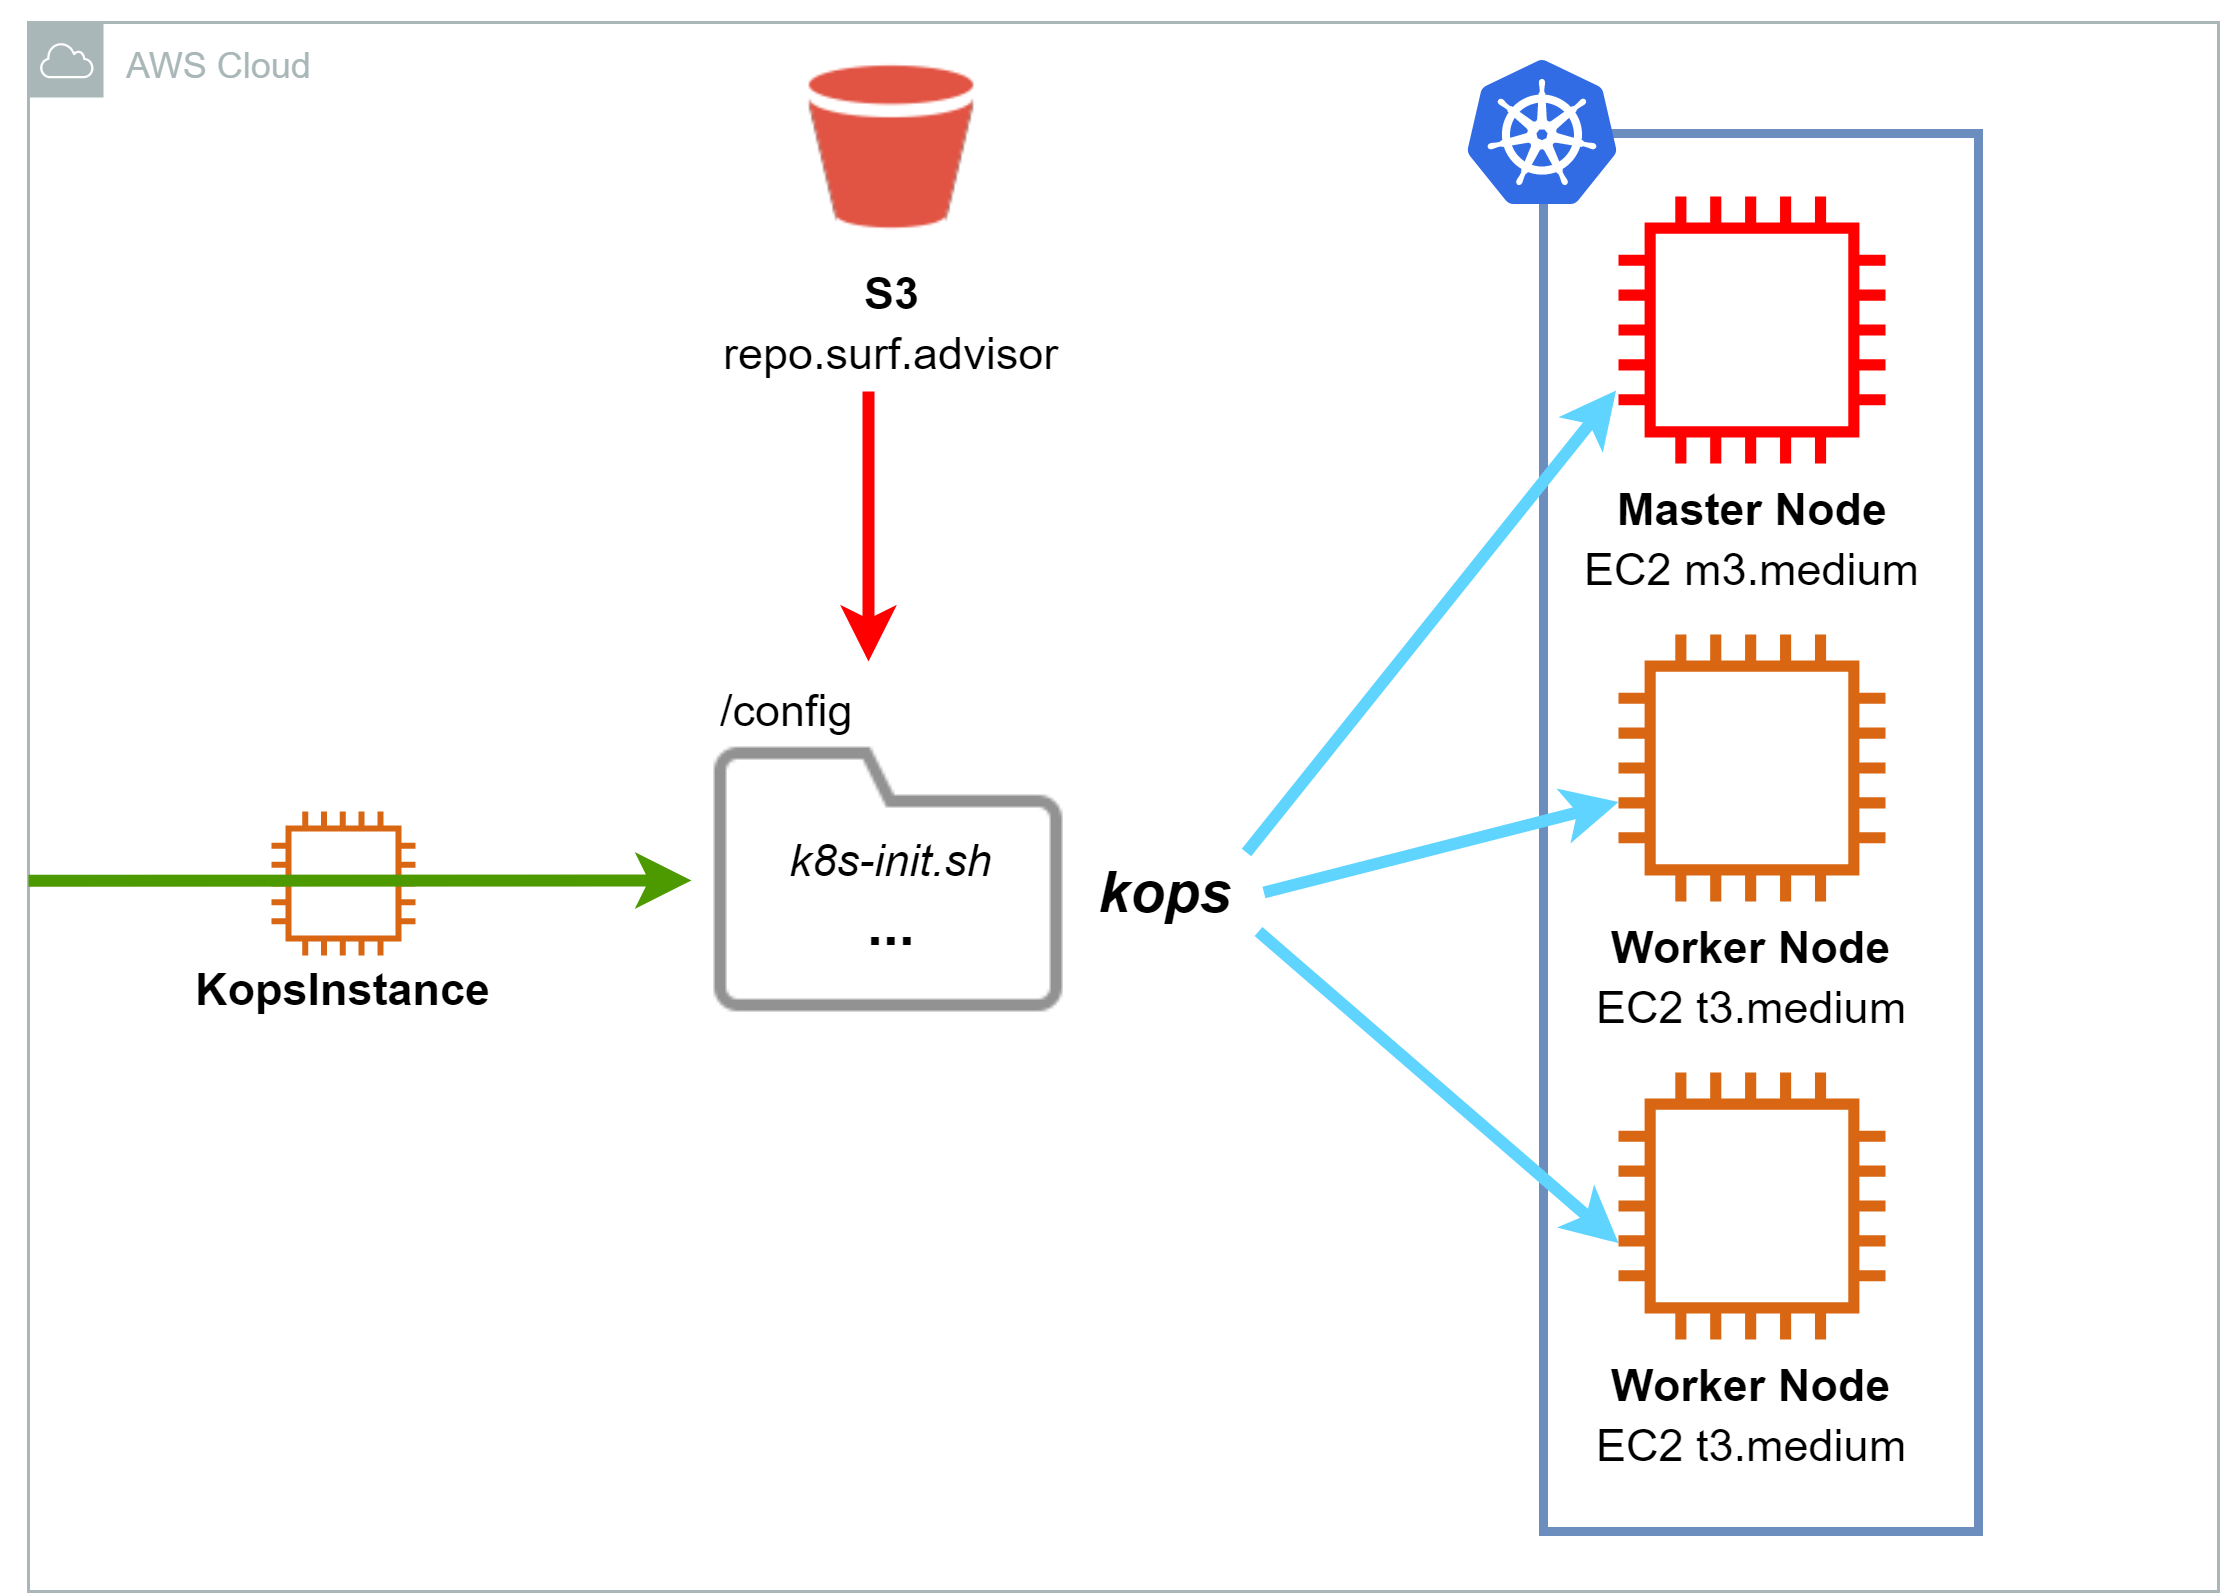
\includegraphics[width=0.95\textwidth]{img/IAC-step2}
	\end{center}
	\caption{Inicjacja Cluter'a SurfAdvisor - 2. Kops}
\end{figure}

\emph{kops} to open-source CLI do budowania \cw{Cluster}'ów Kubernetes na platformie AWS \cite{kops-k8s}.
Stanowi alternatywę dla stosunkowo drogiego na start oficjalnego rozwiązania - EKS \cite{eks-pricing}.

Przy użyciu tego narzędzia dalszy ciąg skryptów, uruchomionych w ramach \emph{UserData} \textbf{KopsInstance} \emph{(\ref{iac:cf})}, buduje \cw{Node}'y składające się na \cw{Cluster}.


\subsection{Kubernetes}
\label{iac:kubectl}

\begin{figure}[!ht]
	\begin{center}
		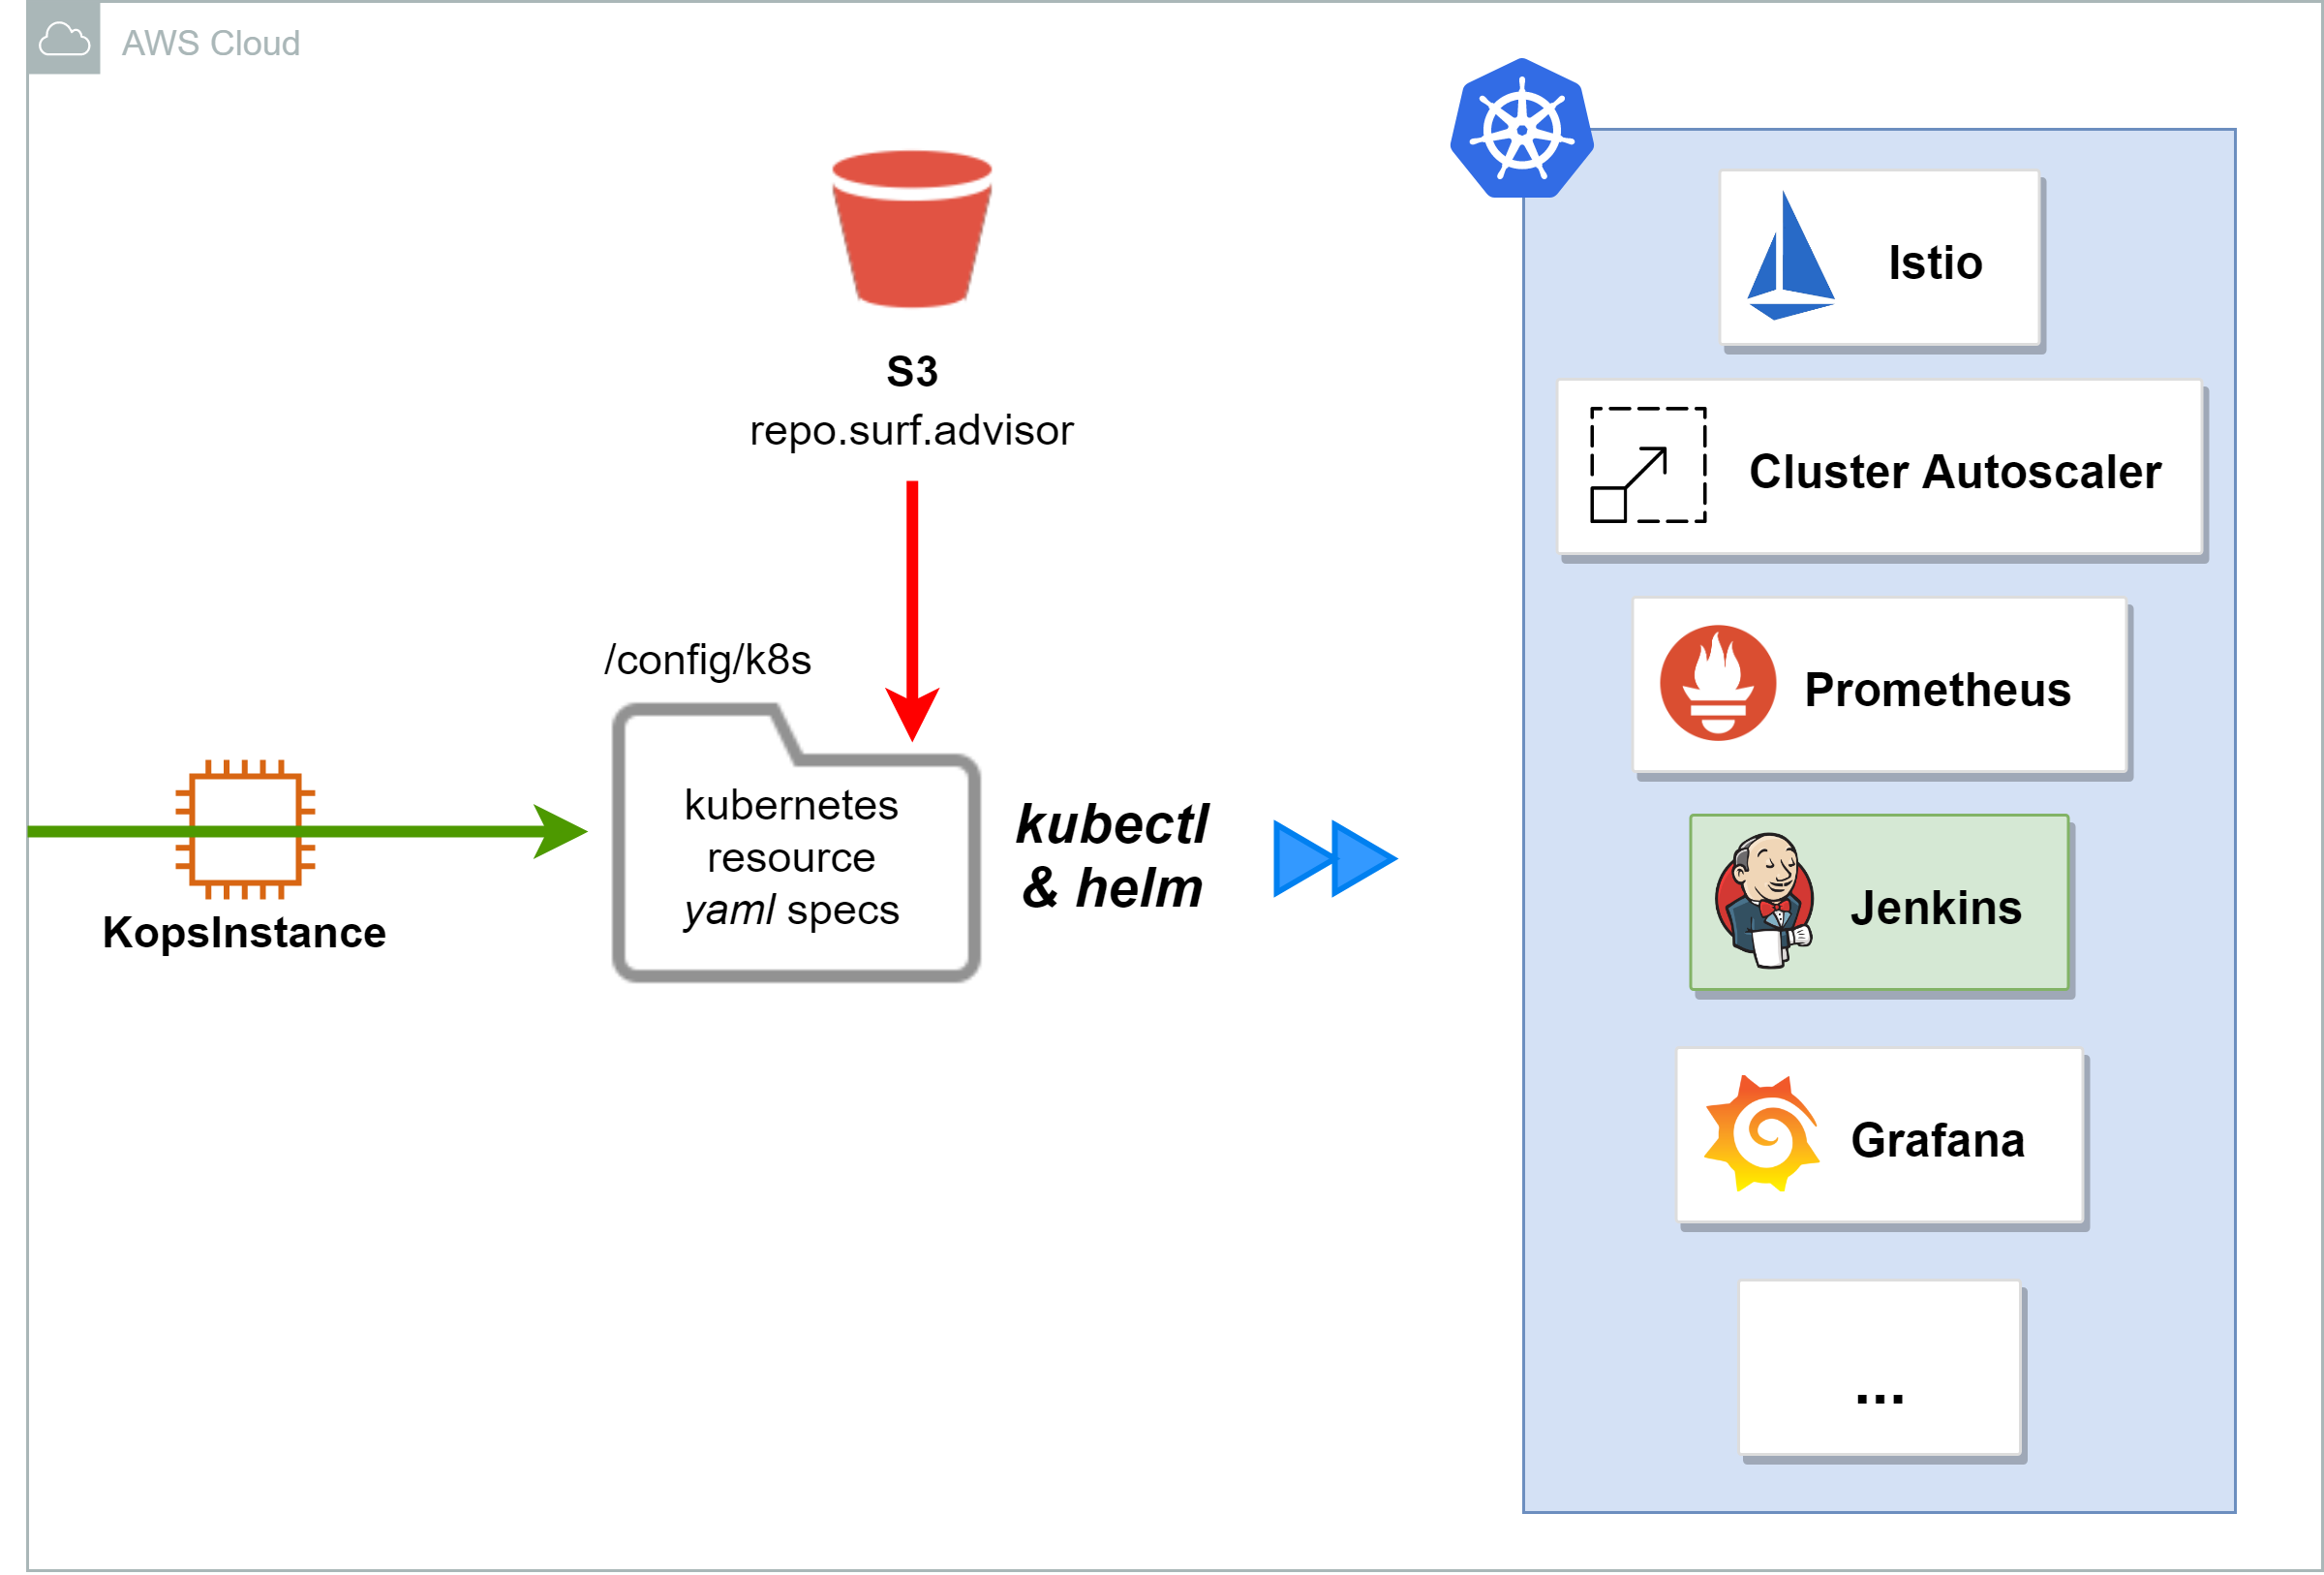
\includegraphics[width=1\textwidth]{img/IAC-step3}
	\end{center}
	\caption{Inicjacja Cluter'a SurfAdvisor - 3. Kubernetes}
\end{figure}

Gdy \emph{kops} skończy już stawiać \cw{Cluster} do akcji wkracza:

\begin{itemize}
    \item
    \emph{\textbf{kubectl}} - oficjalne CLI do operacji na zasobach Kubernetes

    \item
    \emph{\textbf{helm}} - package manager dla Kubernetes
\end{itemize} 

Wdrażane są \cw{Service}'y zaspokajające wymagania bardziej niefunkcjonalne, m.in.:

\begin{itemize}
    \item
    \emph{Jenkins} - który kontynuuje proces inicjacji systemu \emph{[\ref{iac:jenkins}]}

    \item
    \emph{Istio} - sekcja \emph{[\ref{traffic}]}

    \item
    \emph{Prometheus \& Grafana} - sekcja \emph{[\ref{monitoring}]}

    \item
    \emph{Cluster Autoscaler} - rozdział \emph{[\ref{cha:autoscaling}]}
\end{itemize} 


\subsection{Jenkins}
\label{iac:jenkins}

Jenkins jest gotowy do użycia po paru minutach \emph{(wraz ze wszystkimi plugin'ami zdefiniowanymi w pliku konfiguracyjnym)}.
Jedynym manualnym krokiem jaki musimy wykonać jest stworzenie zadania \emph{"Github Organization"}, gdzie podajemy ID naszej organizacji.

\begin{figure}[!ht]
	\begin{center}
		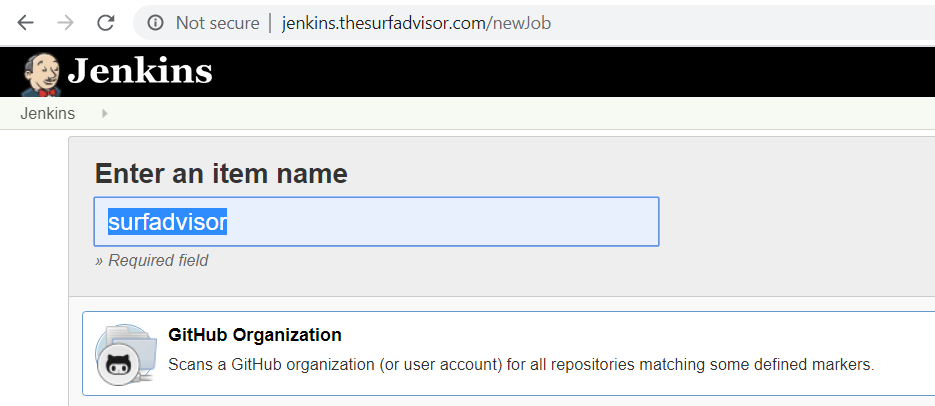
\includegraphics[width=0.8\textwidth]{img/jenkins-new-job}
	\end{center}
	\caption{Jenkins: wdrożenie domenowych serwisów - job "Github Organization"}
\end{figure}

Następnie Jenkins skanuje wszystkie repozytoria widniejące pod daną organizacją i wybiera te zawierące \textbf{\emph{Jenkinsfile}}.
Po chwili będzie dostępna zakładka, na której wylistowane są wszystkie repozytoria spełniające wyżej wymienone kryterium:

\begin{figure}[!ht]
	\begin{center}
		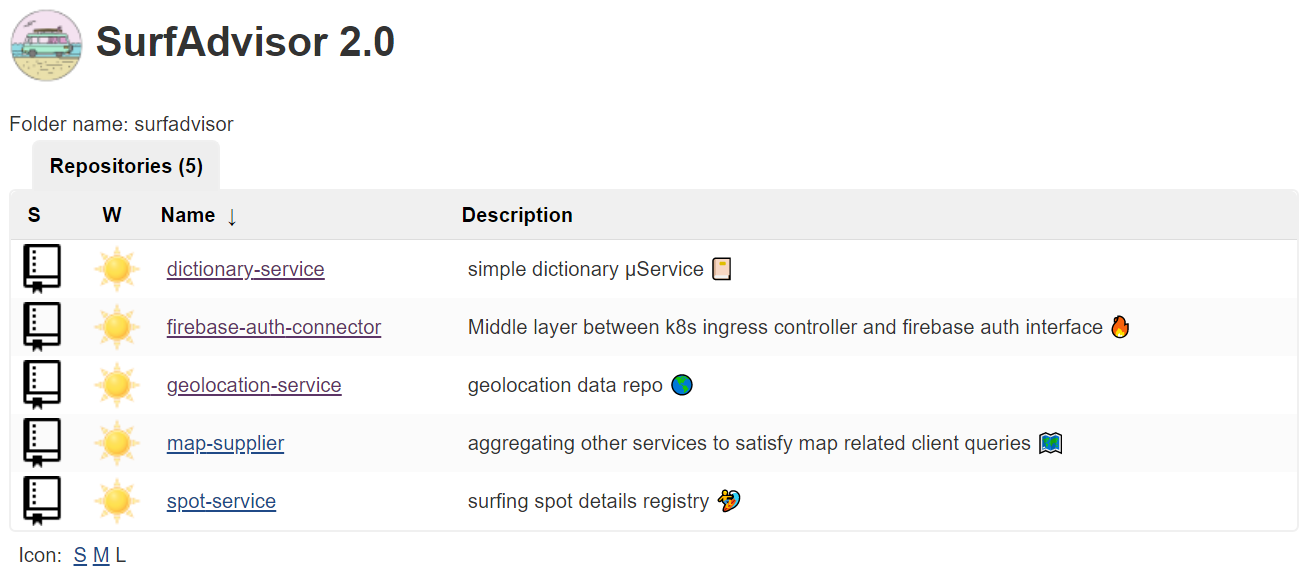
\includegraphics[width=1\textwidth]{img/jenkins-surf-folder}
	\end{center}
	\caption{Jenkins: wdrożenie domenowych serwisów - folder SurfAdvisor}
\end{figure}

Dla każdego z repozytorium Jenkins od razu uruchamia zdefiniowany w \emph{Jenkinsfile} pipeline.
W moim przypadku repozytoria łączy jeszcze obecność dwóch innych plików:
\\\\
\begin{itemize}
    \item
    \emph{\textbf{Dockerfile}} - instrukcja budowy docker image wstawianego potem na DockerHub
    \item
    \emph{\textbf{deploy.yaml}} - deklaracja obiektów Kubernetes: \cw{Service}, \cw{Deployment}, \cw{Pod}, na których stanie dana aplikacja.
    Wdrażane są poprzez \emph{kubectl}.
\end{itemize} 

Poniżej przedstawiony jest wycinek procesowania pipeline dla aplikacji \emph{geolocation-service}.
Dwa końcowe kroki udekorowane są dodatkowo plikiem, na którym polegają.


\begin{figure}[!ht]
	\begin{center}
		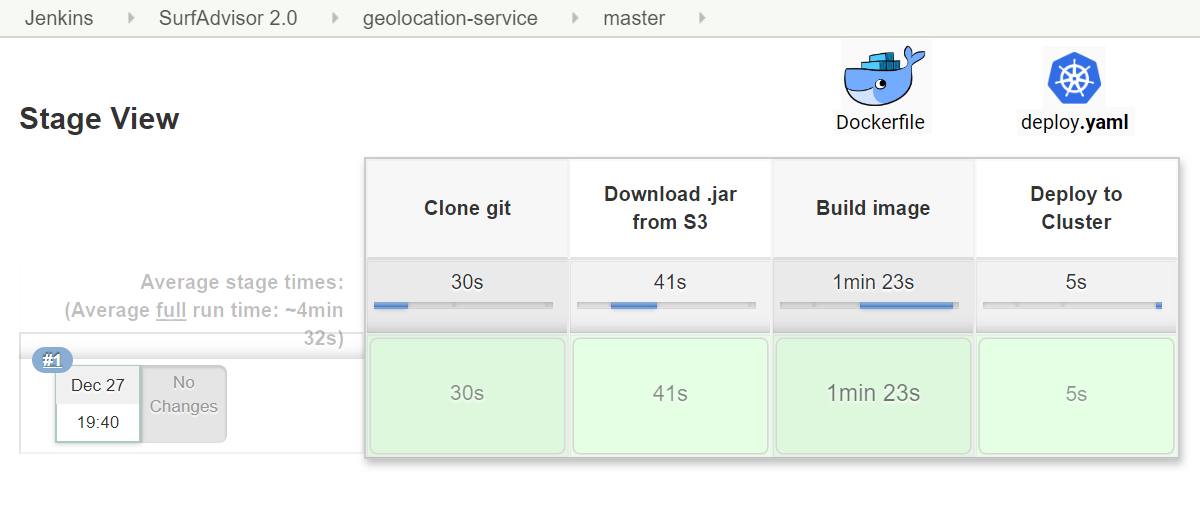
\includegraphics[width=1\textwidth]{img/jenkins-geo-stages}
	\end{center}
	\caption{Jenkins: wdrożenie domenowych serwisów - pipeline}
\end{figure}



 

\section{Zarządzanie ruchem}
\label{traffic}
(2-3s) o rutowaniu i security

\section{Monitoring}
\label{monitoring}
(1-2s) obserwacja parametrów technicznych przy użyciu Prometheus \& Grafana


\section{Realizacja wymagań funkcjonalnych}
(5-10s) Geohash \& Clustering + gdzie i jak to implementuję 
- pochylenie się nad serwisami: geolocation-service, spot-service, map-supplier. 
Prezentacja aplikacji mobilnej